\section{LOGIN}
    Ως \texttt{index.html} ορίζεται η σελίδα Login, στην οποία γίνεται η σύνδεση ή η εγγραφή των χρηστών-πολιτών.
    \begin{figure}[H] \noindent \centering
        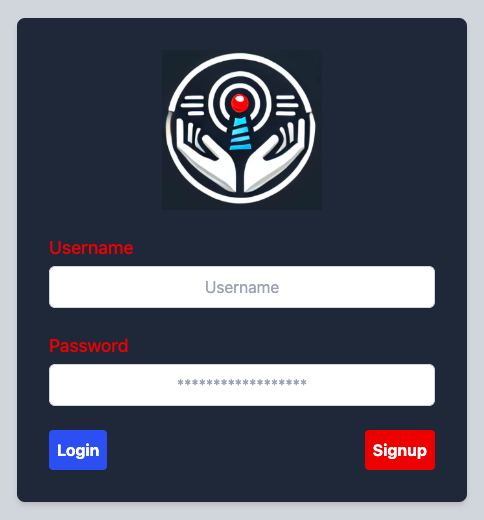
\includegraphics[width=0.3\textwidth]{img/login}
        \caption{Φόρμα Login}
    \end{figure}

    Στη βάση δεδομένων έχουν ήδη δημιουργηθεί κάποιοι λογαριασμοί πολιτών:

    \begin{figure}[H] \noindent \centering
        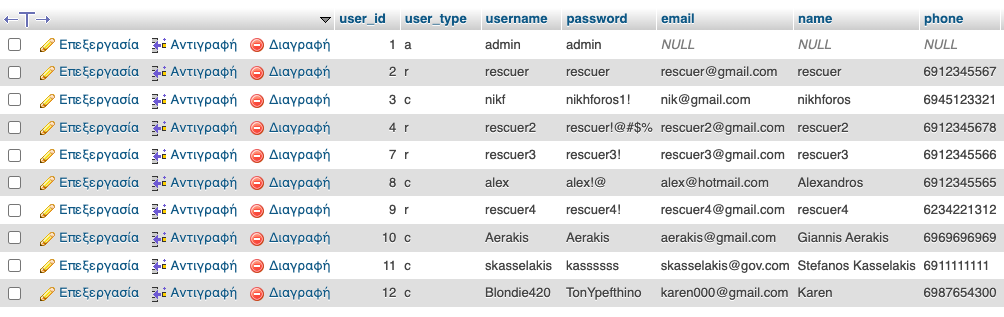
\includegraphics[width=\textwidth]{img/sql-users}
        \caption{πίνακας users}
    \end{figure}

        Η συνάρτηση \textt{login} δέχεται τα ορίσματα των input fields με \texttt{id = #username} και \texttt{id = #password},
            ελέγχεται αν έχουν πληροφορία (αν δεν έχουν, στέλνεται alert μέσω της SweetAlert), και αν έχουν,
            στέλνονται με ένα AJAX request στο \texttt{login.php}.

        Σε περίπτωση επιτυχίας καλείται η \texttt{handleSuccess()}.
        Αυτή, στο αντικείμενο που επιστρέφεται \footnote{redundant, αλλά ελέγχεται αν όντως επιστρέφεται αντικέιμενο· αν όχι εμφανίζεται error},
            ελέγχει το \texttt{user\_type} και κάνει το αντίστοιχο redirect (με ένα delay 2 sec) στην επόμενη σελίδα.

    \subsection{\texttt{login.php}}
        Αφού ανακτήσει το \texttt{username} και \texttt{password} από το AJAX request, στέλνει query στη βάση δεδομένων βάσει του \texttt{username}.
        Αν βρει, ελέγχει εξίσου και το \texttt{password} και στη συνέχεια δημιουργεί ένα array με τις πληροφορίες (\texttt{username}, \texttt{user\_id} και \texttt{user\_type}) του χρήστη, και ένα cookie με διάρκεια 30 ημερών.

        Εν τέλει, στέλνεται με echo ένα JSON αρχείο της μορφής
        \begin{graycomment}
            \verb|[{"username": <...>, "user_id": <...>, "user_type": <"a" ή "r" ή "c">}]|
        \end{graycomment}
